% CS224W Fall 2026 project proposal (project type 1: real-world application of GNNs).
% Compile on Overleaf (upload this file, refs.bib, neurips_2022.sty, figures/) or with latexmk -pdf proposal.tex.
% Before submitting, resolve every "TODO" comment below.

\PassOptionsToPackage{numbers, compress}{natbib}  % numeric citations [1, 2] save space
\documentclass{article}
\usepackage[final]{neurips_2022}                   % [final] shows the author block
\makeatletter                                      % replace the NeurIPS 2022 footer with the course
\renewcommand{\@noticestring}{CS224W: Machine Learning with Graphs, Stanford University, Fall 2026. Project proposal.}
\makeatother

\usepackage[utf8]{inputenc}
\usepackage[T1]{fontenc}
\usepackage{hyperref}
\usepackage{url}
\usepackage{booktabs}
\usepackage{amsmath}
\usepackage{amsfonts}
\usepackage{graphicx}
\usepackage{microtype}

\title{Worth the Lookup: Budgeted Relational Retrieval\\for Call-List Prioritization}

\author{%
  Max Rodriguez\\
  Stanford University\\
  \texttt{SUNETID@stanford.edu}  % TODO: your Stanford email
}

\begin{document}
\maketitle

\noindent\textbf{Project type:} real-world application of GNNs (blog post + Colab).
\textbf{Group:} Max Rodriguez (individual project). % TODO: confirm on Ed that a solo project is approved.

\section{Application domain}

Sales teams work through call lists. Before a rep dials, a research agent can prepare each prospect by looking things up: a contact's recent activity, details about their company, signs of buying intent. Every lookup costs something (an enrichment credit, LLM tokens, or seconds of latency before a parallel dialer connects), so no team researches every prospect in depth. The agent has to decide \emph{which lookups to make for the whole list} within a budget.

This is a graph problem: sales data are linked tables, and different prospects touch the same accounts, events, and activity. Two things couple the prospects on a list. \emph{Shared entities}: enriching one entity informs every prospect connected to it. \emph{A shared ranking cutoff}: a rep calls the top $K$, so a lookup matters only if it could move a prospect across the cutoff, which depends on everyone else's scores. Researching prospects one at a time ignores both.

\textbf{Research question.} Given a call list of $N$ prospects and a budget of $B$ lookups, which lookups should a research agent make so that a graph neural network ranks the list best? We will (i) measure \emph{retrieval-budget frontiers} (ranking quality per lookup spent) for relational GNNs, (ii) train GNNs that stay accurate on partially retrieved neighborhoods, and (iii) compare lookup policies, ending with a learned, batch-aware value model.

\section{Datasets, task, and metrics}

We use RelBench~\cite{robinson2024relbench}, a benchmark of real relational databases with temporal train/validation/test splits and maintained GNN and LightGBM baselines. The data are public: they are hosted openly on Hugging Face (\texttt{stanford-star/relbench-v1}, no login or gating) and were originally released through Kaggle competitions.\footnote{Event Recommendation Engine Challenge and Avito Context Ad Clicks, on kaggle.com.} Our code downloads them; we do not re-host data.

\begin{table}[h]
  \centering
  \small
  \setlength{\tabcolsep}{4pt}
  \begin{tabular}{@{}lllrrrl@{}}
    \toprule
    Dataset / task & Rows (tables) & Label (horizon) & Train / val & Val pos. & GNN / LGBM & Shared \\
    \midrule
    \texttt{rel-event} / \texttt{user-ignore} & 44.8M (5) & ignores $>$2 invitations (7 d) & 19,239 / 2,013 & 11.1\% & 0.804 / 0.773 & events 34\% \\
    \texttt{rel-avito} / \texttt{user-clicks} & 24.7M (8) & clicks $>$1 ad (4 d) & 59,454 / 21,183 & 3.5\% & 0.666 / 0.548 & ads 0.1\% \\
    \texttt{rel-f1} / \texttt{driver-top3} & 97.6K (9) & top-3 qualifying (30 d) & 1,353 / 588 & 20.2\% & 0.680 / 0.649 & -- \\
    \bottomrule
  \end{tabular}
  \caption{Tasks. GNN / LGBM: test AUROC of RelBench's GNN and of LightGBM on the target row only (RelBench leaderboard). Shared: fraction of entities touched by two or more prospects in random 128-prospect lists from the validation day (mean of 200 lists). \texttt{rel-f1} is a small development dataset.}
  \label{tab:data}
\end{table}

\textbf{Why these datasets.} (1)~\emph{Headroom}: the GNN clearly beats a model that sees only the target's own row, so retrieving context matters; we exclude tasks without this gap, such as \texttt{rel-event}/\texttt{user-repeat} (0.686 vs.\ 0.689). (2)~\emph{Contrasting sharing}: on \texttt{rel-event} a third of touched events are shared and a shared cache saves 38\% of event lookups, while on \texttt{rel-avito} only 0.1\% of ads are shared, which tests when joint planning helps. (3)~\emph{Sales analogues}: will a prospect ignore outreach next week, or show intent? Both tasks score many entities at once, like a daily call list, and positives are rare (3.5\% on \texttt{rel-avito}), so ranking the top of the list is what matters.

\textbf{Metrics.} AUROC (RelBench's official metric), average precision, and Precision@$K$ with $K=\lceil 0.1N \rceil$, averaged over random call lists of $N=128$. For budgeted runs we report each metric against lookups per prospect (the frontier) and the area under it. We tune on validation and evaluate on test once.

\section{Graph ML approach}

\textbf{Model.} We use relational deep learning (RDL)~\cite{fey2024rdl}, built with RelBench and PyTorch Geometric~\cite{fey2019pyg}. Each row is a node, each primary--foreign-key link is an edge in both directions, and each row keeps its timestamp $\tau(v)$. Neighbors are sampled over two hops (fanouts 128 and 64) using only rows dated no later than the prediction time $t$. A row $v$ of table $T(v)$ is encoded by a per-table tabular encoder plus a time encoding $\phi$, then updated by heterogeneous GraphSAGE~\cite{hamilton2017sage} over relations $\mathcal{R}$; an MLP head turns the target's final vector into a probability:
\begin{align}
  h_v^{(0)} &= \mathrm{Enc}_{T(v)}(x_v) + \phi\big(t-\tau(v)\big), \\
  h_v^{(\ell+1)} &= \mathrm{ReLU}\Big(\mathrm{LN}\Big(\textstyle\sum_{r\in\mathcal{R}} W^{(\ell)}_{r,1} h_v^{(\ell)} + W^{(\ell)}_{r,2} \sum_{u\in\mathcal{N}_r(v)} h_u^{(\ell)}\Big)\Big).
\end{align}

\textbf{Partial retrieval.} Let $O$ be the set of rows fetched so far. Rows outside $O$ are either removed from message passing or kept as \emph{stubs} with a learned per-table vector:
\begin{equation}
  \tilde h_v^{(0)} = m_v\, h_v^{(0)} + (1-m_v)\, e^{\mathrm{mask}}_{T(v)}, \qquad m_v = \mathbb{1}[v\in O].
\end{equation}
Temporal sampling draws each target's neighborhood separately, so a shared row appears once per target that touches it (in one batch of 8 \texttt{rel-f1} drivers, 629 sampled race rows were only 176 distinct races). We therefore key $O$ on original row ids, so one fetch reveals every copy.

\textbf{Lookups and policies.} There are two actions, each costing one unit: \emph{pull} a prospect's recent rows from one table, or \emph{enrich} an entity referenced by fetched rows. For call list $Q$ with labels $y$ and metric $M$, we seek
\begin{equation}
  \max_{\pi}\ \mathbb{E}\big[M\big(f_\theta(Q \mid O^{\pi}_{B}),\, y\big)\big] \quad\text{s.t.}\quad |O^{\pi}_{B}| - |O_0| \le B.
\end{equation}
Baselines: random; case-local round-robin ($B/N$ lookups per prospect); uncertainty-first; coverage (most-shared entity first); per-prospect acquisition~\cite{norcliffe2025sefa,valancius2024aco}; a singleton-value scorer~\cite{zhou2026scout}; oracle-greedy (uses labels; diagnostic only); and full information. Our policy learns the \emph{batch} value of a lookup, the loss reduction summed over the list, by regression on oracle values from training lists, and applies it greedily:
\begin{equation}
  V(a\mid O)=\textstyle\sum_{i\in Q}\big[\ell\big(f_\theta(q_i\mid O),y_i\big)-\ell\big(f_\theta(q_i\mid O\cup\{a\}),y_i\big)\big].
\end{equation}

\textbf{Why this model fits.} Message passing over foreign keys uses relational data directly, without hand-built aggregates. Temporal sampling prevents label leakage, which a unit test checks. Shared entities are shared rows, so one fetch's value to several prospects is explicit, and stubs separate ``exists but not fetched'' from ``absent''.

\textbf{Related work.} RDL assumes the whole database is available at prediction time; KumoRFM-2 tests random removal of features and links~\cite{hudovernik2026kumorfm2} and STEER prunes context to save compute~\cite{mohamed2026steer}, but neither chooses costed lookups. Active feature acquisition works per instance~\cite{norcliffe2025sefa,valancius2024aco,feng2026brig} or per cohort without shared entities~\cite{rheude2025cama}. The closest graph method values each node query independently on homogeneous dynamic graphs~\cite{zhou2026scout}, and collective active inference acquires labels, not rows~\cite{bilgic2010active}. Stubs build on GNNs with missing features~\cite{rossi2022fp}.

\begin{figure}[t]
  \centering
  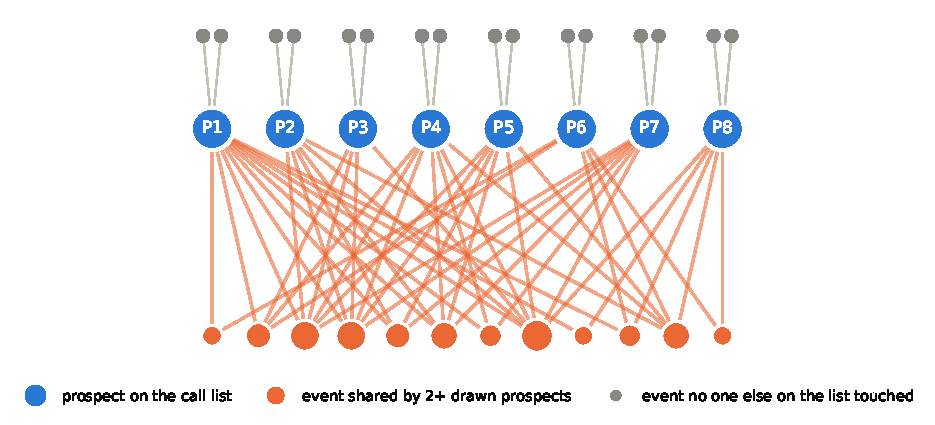
\includegraphics[width=0.72\linewidth]{figures/fig1_call_list.pdf}
  \caption{A real call list as a graph (\texttt{rel-event}, validation day 2012-11-21). From a random list of 128 prospects, the 8 that share the most events with the rest of the list (blue), the 12 most-shared events among them (orange; larger means shared by more of the 8), and two unshared events per prospect (grey). Enriching one orange event informs every prospect connected to it.}
  \label{fig:calllist}
\end{figure}

\section{Evaluation plan and preliminary results}

\textbf{Hypotheses.} H1: the frontier is concave (most of the gap recovered with $\le$25\% of rows). H2: training on partial retrieval helps at low budgets. H3: on \texttt{rel-avito}, past search results (which record past clicks) are the most valuable lookups. H4: batch-aware policies beat case-local ones by more on \texttt{rel-event} than on \texttt{rel-avito}. H5: the learned batch value beats the best heuristic and the singleton scorer. Analyses: frontiers per policy; ablations (training regime, stubs vs.\ removal, batch vs.\ per-prospect credit); architectures (GraphSAGE, GAT, LightGBM); subsets (cold starts, sharing level, list size); and which tables each policy fetches.

% TODO: replace these numbers with your own P7 runs (3 seeds, 20 epochs) before submitting.
\begin{table}[h]
  \centering
  \small
  \begin{tabular}{@{}lccc@{}}
    \toprule
    Validation AUROC on \texttt{rel-f1}/\texttt{driver-top3} & all rows ($p=1$) & 25\% of rows & target row only \\
    \midrule
    LightGBM, target row only & -- & -- & 0.661 \\
    GNN, trained on full neighborhoods & 0.752 $\pm$ 0.020 & 0.749 $\pm$ 0.010 & 0.642 $\pm$ 0.049 \\
    GNN, trained on random partial neighborhoods & 0.734 $\pm$ 0.015 & 0.718 $\pm$ 0.019 & 0.612 $\pm$ 0.025 \\
    \bottomrule
  \end{tabular}
  \caption{Preliminary results. Rows are revealed uniformly at random and hidden rows are removed; mean $\pm$ sd over 3 seeds, 20 epochs each.}
  \label{tab:prelim}
\end{table}

\textbf{Preliminary results.} On the development dataset (Table~\ref{tab:prelim}), the GNN with all rows beats LightGBM on the target row by 0.09 AUROC, and a random quarter of the rows keeps nearly all of that, consistent with H1. Training on random partial views did not help, so H2 is not supported here; we will retest it with stubs, chosen lookups, and the primary datasets. With only the target row, LightGBM (which can use driver names as identity categories) stays ahead. Runs vary by 0.02--0.05 AUROC because PyG's temporal sampler is not seeded, so we report means over at least three seeds.

\textbf{Plan.} Full-information baselines on \texttt{rel-event} and \texttt{rel-avito} on an AWS GPU (by Oct 25); a lookup environment with pull/enrich actions and one shared cache (Nov 1); heuristic frontiers and first tests of H1, H3, and H4 (milestone, Nov 10); the learned batch value and ablations (Nov 24); blog post and Colab (Dec 10).

\small
\bibliographystyle{plainnat}
\bibliography{refs}

\end{document}
